\documentclass[11pt,b5paper,oneside,titlepage,lualatex]{ltjsreport}

%SumatraPDFの逆順検索でエラーが出た時は以下のコマンドラインをSumatraPDFの設定→オプションで入力する
%"C:\Program Files (x86)\TeXstudio\texstudio.exe" "%f" -line %l

\usepackage{luatexja} % ltjclasses, ltjsclasses を使うときはこの行不要
\usepackage[marginparwidth=0pt,margin=10truemm]{geometry}

% --------------------------------------------------------------------------
%		パッケージとコマンド
% --------------------------------------------------------------------------

\usepackage{mypackage} % よく使うパッケージ.
\usepackage{mycommand} % 自分で定義したコマンド. 

% --------------------------------------------------------------------------
%		定理環境
% --------------------------------------------------------------------------

%	パッケージ
\usepackage{tcolorbox} % 定理環境に枠を付けるために必要
\tcbuselibrary{breakable, skins, theorems} % 定理環境に枠を付けるために必要

% 定理番号の設定
\newtcbtheorem[number within=section]{theoremcounter}{Theorem Counter}{}{theoremcounter} % 定理番号のオプションを選択. 
\newtcbtheorem[number within=chapter]{exercisecounter}{Exsercise Counter}{}{exercisecounter} % 演習問題番号のオプションを選択.

% 自作スタイルファイル読み込み
\usepackage{mytheoremcolor} % カラフルな定理環境. 
\usepackage{myprogram} % ハイライト付きソースコード. 

% --------------------------------------------------------------------------
%		ハイパーリンク
% --------------------------------------------------------------------------

%目次にもハイパーリンクが付く. プリアンブルのできるだけ後ろに書く. 
\usepackage[luatex, pdfencoding=auto]{hyperref}
\hypersetup{% hyperrefオプションリスト
	colorlinks=true,
	linkcolor=orange, % リンクの色
	citecolor=cyan, % 引用文献の色
	urlcolor=violet, % URLの色
}

% --------------------------------------------------------------------------
\begin{document}
% --------------------------------------------------------------------------

\title{代数的整数論の道案内}
\author{村上友哉}
\date{\today}
\maketitle


% --------------------------------------------------------------------------

\chapter*{はじめに} \label{chap:intro}
\addcontentsline{toc}{chapter}{はじめに}

% --------------------------------------------------------------------------

この文書は, 代数的整数論をこれから勉強したい人や要点を速習したい人, あるいは勉強したけれど消化不良感がある人のための道案内として書かれたものです. 
証明の細部には立ち入らず, なぜこのようなことを考えるのかというモチベーション, 理論の源泉となる具体的な計算例, 勉強する上で躓きやすいポイントを紹介することに重点を置きます. 
他の本(例えば\cite{Yukie1}, \cite{Yukie2}, \cite{Neu})で勉強する際の副読本として利用してもらえればと思います. 

この文書ではどのような前提知識を課すか, ということについて述べておきます. 
この文書を\textbf{読み始める}ための前提知識は特に課しません. 
と言うより, 前提知識が無くても読み始めることはできるように気を付けて書いた, と言う方が正確です. 
実際, この文書では方程式の整数解のような中高生にも親しみやすい概念から話を進めていきます. 
一方で, この文書を\textbf{読み進める}ための前提知識は色々と必要なものがあります. 
というのも, 代数的整数論について証明抜きで紹介していく以上, そこで用いられる理論(群論, 環論, 体論, 線形代数などなど)の助けを借りた説明になってしまうのはどうしても避けられないからです. 
ですが, それらの知識をまず身に付けてからこの文書を読む(あるいは代数的整数論を勉強する)というのではなく, まずはこの文書を読み進めてみて, どこかで知識の壁を感じたら一旦知識を補填して, そしてまたこの文章に戻る(あるいは代数的整数論の勉強に戻る)という風にするのが効率も良く身に付きやすい勉強法なのではないかと思います. 


\begin{quote}
	\centering
	[工事中]
\end{quote}


% --------------------------------------------------------------------------

\section*{謝辞}

% --------------------------------------------------------------------------

この文書の内容は2021年5月から筆者が主催したセミナーに基づきます. 
庄司幸弘さん, 前畑佑都さん, 田中拓弥さんにはセミナーに参加し質問やコメントを頂きました. 
特に前畑佑都さんには演習問題の作成に役立つ計算例を提示して頂きました. 
小野雅隆さんには数学的な誤りを, 川村悟史さんには数学的な誤りと誤植をご指摘頂きました. 
ここに感謝いたします. 

\clearpage

\tableofcontents
%\addcontentsline{toc}{chapter}{目次}

% --------------------------------------------------------------------------

\chapter{代数的整数論とは?} \label{chap:代数的整数論とは}

% --------------------------------------------------------------------------




% --------------------------------------------------------------------------

\section{代数的整数論の研究対象} \label{sec:代数的整数論の研究対象}

% --------------------------------------------------------------------------

\begin{quote}
	\centering
	代数的整数論とは何か?
\end{quote}
この問いに答えるのが本章の目的です. 

さっそく答えを言ってしまうと, 
\begin{quote}
	\centering
	代数的整数論とは, \textbf{代数的整数}の理論である
\end{quote}
というのが一つの答えです. 
では\textbf{代数的整数}とは何か?\,
定義を見てみましょう. 

\begin{dfn}{}{}
	複素数$ \alpha $が\textbf{代数的整数}であるとは, ある整数係数多項式$ f(x) = x^n + a_1 x^{n-1} + \cdots + a_n $が存在して$ f(\alpha) = 0 $を満たすことを言う. 
\end{dfn}

定義のポイントは$ f(x) $が$ x^n $から始まる多項式であるところです. 
このような多項式を\textbf{モニック多項式}と呼びます. 
この用語を用いると, 代数的整数とは「整数係数モニック多項式の根」のことだと言い換えることができます. 

\begin{exc}{}{}
	代数的整数論の本で代数的整数の定義を確認しましょう. 
\end{exc}

では, この代数的整数という概念について理解を深めるために例を見ていきましょう. 

\begin{ex}{}{alg_num}
	整数は代数的整数である. また$ \sqrt{2}, \sqrt{-1}, e^{2\pi \iu/5} $は代数的整数である. 
\end{ex}

\begin{exc}{}{}
	\exref{alg_num}で挙げた代数的整数の例について, それを根に持つような整数係数モニック多項式を挙げましょう. 
\end{exc}

\begin{exc}{}{}
	\exref{alg_num}で挙げた以外の代数的整数の例を挙げましょう. 
\end{exc}

さて, 以上のことをまとめると
\begin{quote}
	\centering
	代数的整数論とは, $ \sqrt{2} $や$ \sqrt{-1} $などの代数的整数を研究する理論である
\end{quote}
と述べることができます. 

となると, 代数的整数は研究するに値する対象なのか, どのような応用があるかということが気になる方もいると思います. 
実は, 代数的整数は方程式の整数解を調べるのに役立ちます. 
詳しいことは次章以降で説明しますが, 核となるアイデアを具体例に沿って述べると, 例えば$ x^2 - 2y^2 = 1 $という方程式は
$  \left(x - \sqrt{2}y \right) \left(x + \sqrt{2}y \right) = 1 $という風に言い換えることができるので, $ \sqrt{2} $という数の性質からこの方程式を調べることができるのです. 
このため, 代数的整数論の応用として種々の方程式の整数解を求めることができます. 
このことについてはこの文書の随所で様々な具体例を示します. 

%そのような観点からは
%\begin{quote}
%	\centering
%	代数的整数論とは, 方程式の整数解を研究する理論である
%\end{quote}
%とより素朴に言い換えることもできます. 

% --------------------------------------------------------------------------

\section{代数的整数論の目的} \label{sec:代数的整数論の目的}

% --------------------------------------------------------------------------

前節では「代数的整数論では代数的整数を調べる」という話をしました. 
とは言ったものの, 実際の代数的整数論ではそこまで代数的整数や方程式それ自体をガシガシ弄るわけではありません. 
実際の代数的整数論の主目的は, \textbf{代数体の整数環}の\textbf{素イデアル}の\textbf{分解}や\textbf{分布}を調べることです. 
……専門用語が色々出てきました. 
これらの専門用語の説明は後の章に回すことにして, ここではなぜ実際の代数的整数論が代数的整数ではなくそのような難しそうな概念(実際, これらは代数的整数よりも抽象度の高い概念です)を調べるのかということを説明してみたいと思います. 

実は, より抽象度の高い概念を追求するということは数学ではよくあることです. 
このことをGalois理論を例にとって説明してみたいと思います(Galois理論を勉強したことが無い方は, 以下の話はそういうものかと読み流してください). 

19世紀の数学者Galoisによって見出されたGalois理論は, 
\begin{quote}
	\centering
	方程式$ x^n + a_1 x^{n-1} + \cdots + a_n = 0 $(ただし$ a_i \in \Q $)
	
	を調べる代わりに
	
	\textbf{体}$ \Q(\alpha) $(ただし$ \alpha $は方程式$ x^n + a_1 x^{n-1} + \cdots + a_n = 0 $の解の1つ)やその\textbf{Galois群}
	
	を調べる!
\end{quote}
というパラダイムシフト(視点の転換)を引き起こしました. 
つまり, 方程式を調べたければ, (数学的により洗練された対象である)体やそのGalois群を代わりに調べれば良い, という革命的な視点を提供したのです. 
この革命が当時の数学界に与えた反響が非常に大きかったことは想像に難くないですが, Galois理論が定着するにつれ, いつしか興味は方程式から(より本質的な対象である)体へと移っていきました. 
Galois理論の教科書に「これって方程式とどう関係するの?」と首をかしげたくなるような命題がつらつらと並んでいるのはそのためです. 

実は, 代数的整数論でもGalois理論と同じようなパラダイムシフトが起こっています. つまり
\begin{quote}
	\centering
	%方程式の整数解(例えば$ x^n + y^n = z^n $)や
	代数的整数(例えば$ \sqrt{2} $)
	
	を調べる代わりに
	
	\textbf{代数体の整数環}(例えば$ \Z[\sqrt{2}] $)やその\textbf{素イデアル}
	
	を調べる!
\end{quote}
という視点の切り替えがあったのです. 
これにより, いつしか興味は方程式の整数解から(より数学的に洗練されていて本質的な対象である)\textbf{代数体の整数環}やその\textbf{素イデアル}へと移りました. 
このような背景から代数的整数論では代数体の整数環や素イデアルといったより抽象的な概念を調べていて, そのために代数的整数論の教科書は内容が厳つくなってしまうのです. 
その一方で抽象度が高い概念を調べるがゆえに, 理論が美しく整然としているのもまた事実です. 

\clearpage




% --------------------------------------------------------------------------

\chapter{代数体の整数環の動機} \label{chap:代数体の整数環の動機}

% --------------------------------------------------------------------------

\ref{sec:代数的整数論の研究対象}節の最後で
\begin{quote}
	\centering
	代数的整数は方程式の整数解を調べるのに役立ち, そのため代数的整数論の応用として種々の方程式の整数解を求めることができる
\end{quote}
ということを述べました. 
一方\ref{sec:代数的整数論の目的}節では
\begin{quote}
	\centering
	実際の代数的整数論で調べるのは代数体の整数環などのより抽象的な概念である
\end{quote}
ということを述べました. 
これらのことを踏まえて, 本章では
\begin{quote}
	\centering
	なぜ代数体の整数環を考えるのか?
\end{quote}
という問いに答えたいと思います. 
本章の目的は, 
\begin{quote}
	\centering
	代数体の整数環を調べると嬉しいことが色々あるんだな, じゃあ一丁, 調べてやりますか
\end{quote}
という気持ちになってもらうことです. 
そのためにまず\ref{sec:Fermatの最終定理と一意分解整域}節でFermatの最終定理, \ref{sec:Pell方程式と単元}節でPell方程式について考察して, 代数体の整数環というものを考えるとこれらの方程式の整数解を見通し良く決定できることを紹介します. 
その後\ref{sec:代数体の整数環の定義と例}節で代数体の整数環の定義と例について見ていくことにします. 

% --------------------------------------------------------------------------

\section{Fermatの最終定理($ n=3 $)と一意分解整域} \label{sec:Fermatの最終定理と一意分解整域}

% --------------------------------------------------------------------------

本節ではFermatの最終定理の$ n=3 $の場合, つまり次の事実の見通しの良い証明について検討します. 

\begin{thm}{}{}
	$ x^3 + y^3 = z^3 $を満たす自然数の組$ (x, y, z) \in \Z_{>0}^3 $は存在しない.
\end{thm}

ここでは\cite[系8.7.6]{Yukie1}の証明を念頭に置いて話を進めていきますが, 証明を読んでいなくても問題ありません. 

証明の方針は解$ (x, y, z) \in \Z_{>0}^3 $が存在すると仮定して無限降下法で矛盾を導くというものですが, 実際に矛盾を導くための核となるアイデアは以下の通りです. 

\begin{simplesquarebox}{アイデア}
	まず$ \gcd(x, y, z) = 1 $として良いことに注意する. 
	ここで$ \zeta_3 = (-1+\sqrt{-3})/2 $とおくと
	\[
	z^3 = x^3 + y^3 = (x + y) (x + \zeta_3 y) (x + \zeta_3^2 y)
	\]
	と因数分解できる. 
	このとき各$ i \in \{ 0, 1, 2 \} $に対し整数$ u_i, v_i \in \Z $が存在して
	\[
	x + \zeta_3^i y = (u_i + \zeta_3 v_i)^3
	\]
	と書けるのではないか?
\end{simplesquarebox}

最後の推論がこのアイデアの核心的な部分で, これは次の整数の性質からの類推です. 

\begin{lem}{}{}
	どの2つも互いに素な3つの自然数の積が立方数なら, それらは全て立方数である. 
	すなわち, 自然数$ n_1, n_2, n_3, N \in \Z_{>0} $が
	\[
	\gcd(n_1, n_2) = \gcd(n_2, n_3) = \gcd(n_3, n_1) = 1, \quad
	n_1 n_2 n_3 = N^3
	\]
	を満たすなら, 各$ i \in \{ 1, 2, 3 \} $に対し整数$ u_i \in \Z $が存在して$ n_i = u_i^3 $を満たす. 
\end{lem}

代数的整数論とは少し外れますが, 理解の助けにするために証明をつけておきます. 
整数問題に自信のある方はぜひ自力での証明に挑戦してみてください. 

\begin{proof}
	各$ i \in \{ 1, 2, 3 \} $に対し$ n_i = p_{i, 1}^{e_{i, 1}} \cdots p_{i, r_i}^{e_{i, r_i}} $を素因数分解とすると, 
	$ \gcd(n_1, n_2) = \gcd(n_2, n_3) = \gcd(n_3, n_1) = 1 $より
	\[
	N^3 = \left( p_{1, 1}^{e_{1, 1}} \cdots p_{1, r_1}^{e_{1, r_1}} \right) \left( p_{2, 1}^{e_{2, 1}} \cdots p_{2, r_2}^{e_{2, r_2}} \right) \left( p_{3, 1}^{e_{3, 1}} \cdots p_{3, r_3}^{e_{3, r_3}} \right)
	\]
	は$ N^3 $の素因数分解である. 
	よって全ての$ e_{i, j} $は3の倍数なので, $ n_1, n_2, n_3 $は全て立方数である. 
\end{proof}

証明のポイントは整数が素因数分解できることにあります. 
そこで, 上に述べたアイデアを正当化させるには$ x + y\zeta_3 $(ただし$ x, y \in \Z $)という数の体系に対して素因数分解を樹立する必要が出てきます. 
ここで
\[
\Z[\zeta_3] := \{ x + y\zeta_3 \mid x, y \in \Z \}
\]
とおくと, これは足し算と掛け算で閉じており, \textbf{環}と呼ばれる数学的対象になっていることが分かります. 
このとき$ \Z[\zeta_3] $という数の体系に対する素因数分解は, 環論の用語を用いることで次のように定式化することができます. 

\begin{thm}{\cite[定理8.6.1]{Yukie1}}{}
	$ \Z[\zeta_3] $は\textbf{一意分解整域}である.
\end{thm}

そしてこの性質を用いることで, 上で述べたアイデアを遂行してFermatの最終定理の$ n=3 $の場合に証明を与えることができるのです. 

以上の議論では, 
\begin{quote}
	\centering
	方程式の代わりに\textbf{環}を調べる!
\end{quote}
というパラダイムシフトが起こっています. 
そして実のところ, ここで登場した$ \Z[\zeta_3] $という環は代数体の整数環の例になっています. 

以上が, 方程式の整数解の研究に代数体の整数環が役立つことの第一の例です. 

\begin{exc}{}{}
	\begin{enumerate}
		\item $ \alpha, \beta \in \Z[\zeta_3] $に対し$ \alpha \beta \in \Z[\zeta_3] $を示せ. 
		\item 数学書で\textbf{環}の定義を確認し, $ \Z[\zeta_3] $が環をなすことを確認せよ. 
	\end{enumerate}
\end{exc}

% --------------------------------------------------------------------------

\section{Pell方程式と単元} \label{sec:Pell方程式と単元}

% --------------------------------------------------------------------------

次に, 方程式の整数解の研究に代数体の整数環が役立つことの第二の例であるPell方程式について述べたいと思います. 
Pell方程式とは, 平方数でない$ d \in \Z_{>0} $に対する$ x^2 - dy^2 = \pm 1 $という形の方程式を指します. 
ここでは$ d = 2 $の場合を考察してみます. 

$ x^2 - 2y^2 = -1 $という方程式は, いくつか代入してみることで$ (x, y) = (1, 1) $という解を持つことが分かります. 
同様に$ x^2 - 2y^2 = 1 $という方程式は$ (x, y) = (3, 2) $という解を持つことが分かります. 
これらの他にはどのような解があるでしょうか?

実は, これらの解から新しい解を作ることができます. 
そのためには, \ref{sec:代数的整数論の研究対象}節の最後に少しだけ述べた
\[
\pm1 = x^2 - 2y^2 = \left(x - \sqrt{2}y \right) \left(x + \sqrt{2}y \right)
\]
という因数分解を用いることで計算の見通しが立ちやすくなります. 
例えば
\begin{align}
	-1 &= (-1)^3 
	= \left(1 - \sqrt{2} \right)^3 \left(1 + \sqrt{2} \right)^3 
	= \left(11 - 5\sqrt{2} \right) \left(11 + \sqrt{2} \right), \\
	1 &= 1^2 
	= \left(3 - 2\sqrt{2} \right)^2 \left(3 + 2\sqrt{2} \right)^2 
	= \left(17 - 12\sqrt{2} \right) \left(17 + 12\sqrt{2} \right), \\
\end{align}
と計算できるので, 
$ x^2 - 2y^2 = -1 $の解として$ (x, y) = (11, 5) $が, 
$ x^2 - 2y^2 = 1 $の解として$ (x, y) = (17, 12) $があることが分かります. 
ここで
\[
1 = (-1)^2 = \left( \left(1 - \sqrt{2} \right) \left(1 + \sqrt{2} \right) \right)^2
=  \left(3 - 2\sqrt{2} \right) \left(3 + 2\sqrt{2} \right)
\]
であることに注意すると, 結局$ \left(1 + \sqrt{2} \right)^n $を計算することにより, 
$ n $が奇数の時は$ x^2 - 2y^2 = -1 $の解が, 
$ n $が偶数の時は$ x^2 - 2y^2 = 1 $の解が得られることが分かります. 
以上の計算はもちろん$ \sqrt{2} $を出さずに行うこともできますが, $ \sqrt{2} $を出した方が見通しが良いように思います. 

さて, ここで
\begin{quote}
	\centering
	$ \left(1 + \sqrt{2} \right)^n $を計算することで方程式$ x^2 - dy^2 = \pm 1 $の\textbf{全ての}解を得られるか?
\end{quote}
という疑問が浮かび上がりますが, 答えは「YES」です. 
実際, 次の定理が成り立ちます. 

\begin{thm}{}{Pell_2}
	方程式$ x^2 - 2y^2 = 1 $, $ x^2 - 2y^2 = -1 $の解全体の集合はそれぞれ
	\begin{align}
		&\left\{ (x, y) \in \Z^2 \relmiddle{|} x + \sqrt{2}y = \pm \left(1 + \sqrt{2} \right)^n, \text{$ n \in \Z $は偶数} \right\}, \\
		&\left\{ (x, y) \in \Z^2 \relmiddle{|} x + \sqrt{2}y = \pm \left(1 + \sqrt{2} \right)^n, \text{$ n  \in \Z $は奇数} \right\}
	\end{align}
	と表される. 
\end{thm}

この定理は次のように一般化されます. 

\begin{thm}{}{Pell_general}
	平方数でない$ d \in \Z_{>0} $に対し, 
	方程式$ x^2 - dy^2 = \pm 1 $の解全体の集合はある整数の組$ (x_0, y_0) $を用いて
	\[
	\left\{ (x, y) \in \Z^2 \relmiddle{|} x + \sqrt{d}y = \pm \left(x_0 + \sqrt{d}y_0 \right)^n, n \in \Z \right\}
	\]
	と表される. 
\end{thm}

\begin{rem}{}{}
	平方数でない$ d \in \Z_{>0} $に対し, 一般には方程式$ x^2 - dy^2 = -1 $には解が無いことがあるため, \thref{Pell_general}では\thref{Pell_2}とは少し異なる書き方をした. 
	なお, 方程式$ x^2 - dy^2 = 1 $には常に無限個の解が存在する. 
\end{rem}

では, これらの定理はどのように示されるのでしょうか. 
\thref{Pell_2}は初等的に示すことができるのですが, \thref{Pell_general}の証明は難しいです(これは$ \Z[\sqrt{2}] $が単項イデアル整域(より強くEuclid整域)であることと, 一般に$ \Z[\sqrt{d}] $は単項イデアル整域とは限らないことの現れです). 
証明のためにどのようにアプローチするかというと, ここでも方程式$ x^2 - dy^2 = \pm 1 $の代わりに\textbf{環}$ \Z[\sqrt{d}] $を考察するのです. 
そして, $ \Z[\sqrt{d}] $は$ d \equiv 2, 3 $のときには\textbf{代数体の整数環}という対象になっているのです($ d \equiv 1 $の場合は代数体の整数環より少し広いクラスである代数体の整環と呼ばれるものになっていて, 代数体の整数環と並行した議論がある程度できます). 

それでは, Pell方程式を環の言葉で翻訳してみましょう. 
以下では平方数でない$ d \in \Z_{>0} $を固定して議論することにします. 
まずノルム写像を
\[
\begin{array}{cccl}
	N \colon & \Z[\sqrt{d}] & \longrightarrow & \Z \\
	& x + \sqrt{d}y & \longmapsto & \left(x - \sqrt{d}y \right) \left(x + \sqrt{d}y \right)
\end{array}
\]
によって定めます. 
このとき
\[
\begin{array}{ccl}
	\{ (x, y) \in \Z^2 \mid x^2 - dy^2 = \pm 1 \} & \longrightarrow & \{ \alpha \in \Z[\sqrt{d}] \mid N(\alpha) = \pm 1 \} \\
	(x, y) & \longmapsto & x + \sqrt{d}y
\end{array}
\]
は全単射であることがノルム写像の定義から従います. 
このようにしてPell方程式の解集合を環$ \Z[\sqrt{d}] $とノルム写像の言葉で翻訳することができました. 

ここからは環サイドから考察していくことにしましょう. 
まず, 代数的整数論の基礎事項から次の事実を示すことができます. 

\begin{lem}{}{}
	\[
	\{ \alpha \in \Z[\sqrt{d}] \mid N(\alpha) = \pm 1 \}
	= \Z[\sqrt{d}]^\times.
	\]
\end{lem}

ここで$ \Z[\sqrt{d}]^\times $は環$ \Z[\sqrt{d}] $の単元全体のなす集合を表します. 
このようにして, Pell方程式の解集合を環$ \Z[\sqrt{d}] $の単元という理論的により洗練された対象で置き換えることができました. 

\begin{exc}{}{}
	環の単元の定義を, 何も見ずノートに書けるようになりましょう. 
\end{exc}

次に, \textbf{Dirichletの単数定理}という代数的整数論の偉大な結果から次が従います. 

\begin{thm}{}{}
	ある単数$ \veps_0 \in \Z[\sqrt{d}]^\times $が存在して
	\[
	\Z[\sqrt{d}]^\times = \{ \pm \veps_0^n \mid n \in \Z \}
	\]
	が成り立つ. 
\end{thm}

以上の事実から\thref{Pell_general}が従います. 

\begin{exc}{}{}
	上で述べた事実の帰結として\thref{Pell_general}が得られることを示しましょう. 
\end{exc}

ここでの議論は
\begin{itemize}
	\item まずPell方程式を環論的に言い換え, 
	\item 次に代数的整数論の力を使って環を調べる
\end{itemize}
と要約することができます. 
ポイントは, 方程式の代わりに代数体の整数環(と整環)というより洗練された対象を考察するという部分です. 
\ref{sec:Fermatの最終定理と一意分解整域}節と同様, 方程式の整数解の研究に代数体の整数環が役立つことを見て取ることができました. 

\begin{exc}{}{}
	Pell方程式$ x^2 - 3y^2 = \pm 1, x^2 - 27dy^2 = \pm 1 $の解を調べるにはそれぞれどのような環を調べることが有効か述べましょう. 
\end{exc}

% --------------------------------------------------------------------------

\section{代数体の整数環の定義と例} \label{sec:代数体の整数環の定義と例}

% --------------------------------------------------------------------------

\ref{sec:Fermatの最終定理と一意分解整域}, \ref{sec:Pell方程式と単元}節では代数体の整数環を研究することで嬉しいこと(方程式の整数解について理解できること)があると述べました. 
ですがまだ代数体の整数環の定義を述べていませんでしたので, ここで述べたいと思います. 

まず代数体の定義を与えます. 

\begin{dfn}{}{}
	代数体とは$ \Q $の有限次拡大体(となる$ \bbC $の部分体)のことである. 
\end{dfn}

\begin{ex}{}{alg_fld}
	$ \Q(\sqrt{2}), \Q(\iu), \Q(e^{2\pi\iu/5}) $は代数体である. 
\end{ex}

\begin{exc}{}{}
	\exref{alg_fld}で述べた以外の代数体の例を挙げよ. 
\end{exc}

次に代数体の整数環の定義を述べます. 

\begin{dfn}{}{}
	代数体$ K $の整数環$ \calO_K^{} $を
	\[
	\calO_K^{} := \{ \alpha \in K \text{ : 代数的整数} \}
	\]
	と定義する. 
\end{dfn}

\begin{ex}{}{}
	代数体$ \Q(\sqrt{2}) $の整数環は$ \Z[\sqrt{2}] $である. 
	また代数体$ \Q(\sqrt{-3}) $の整数環は$ \Z[\sqrt{-3}] $ではなく$ \Z[(-1+\sqrt{-3})/2] $である. 
	しかしこれらの事実を証明するには, 代数体の全ての元に対しそれが代数的整数かどうか判定する必要があるので少々努力を要する. 
\end{ex}

つまり代数体$ K $の整数環とは, $ K $の元のうち代数的整数であるものを取れるだけとってきたものだということができます. 
%環論の用語を使うと, 代数体の整数環とは代数的整数のなす整閉整域だと換言することもできます. 

\begin{rem}{}{}
	$ \calO $(カリグラフィーのO)とは不思議な記号だが, 実はこの記号は複素多様体論で正則関数のなす環を表すのに用いられ, その記号法はここで述べた代数体の整数環の記号と整合性があることをスキーム論の観点から理解することができる. 
\end{rem}

\begin{figure}[hbtp]
	\centering
	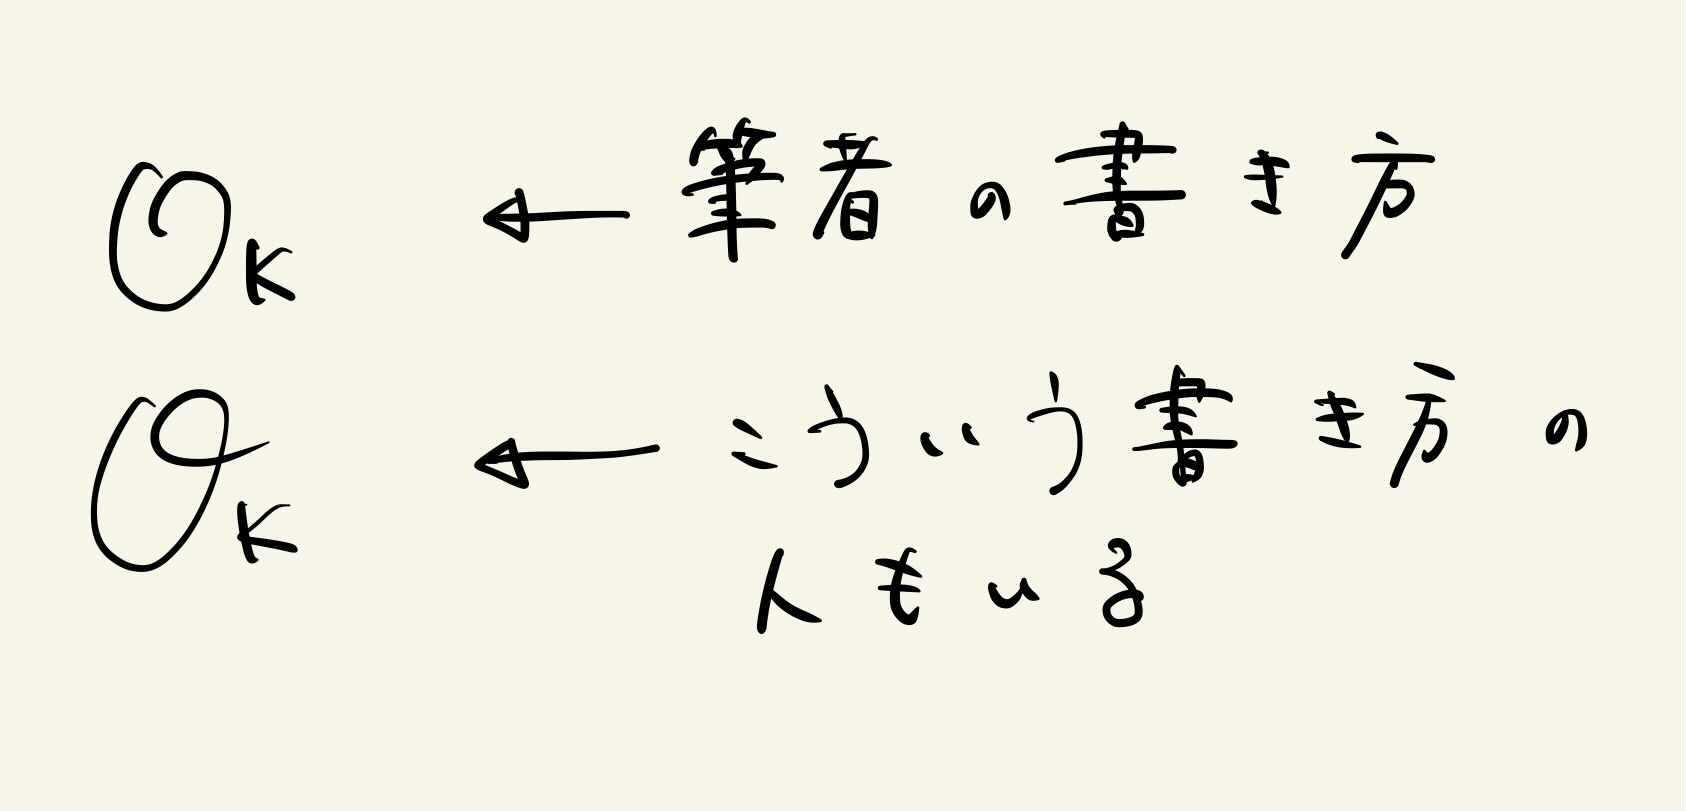
\includegraphics[clip,width = 5.0cm]{O_K.jpg}
	\caption{手書きの$ \calO_K^{} $}
\end{figure}

\clearpage

% --------------------------------------------------------------------------

\chapter{イデアルとDedekind環の動機} \label{chap:イデアルとDedekind環の動機}

% --------------------------------------------------------------------------

前章では, 方程式の整数解を調べるには代数体の整数環を調べることが有効であるということを述べました. 
しかしながら, 様々な種類の方程式の整数解を調べるためには一筋縄ではいかず, 代数体の整数環のより深い性質を理解することが必要になってきます. 

本章では, \ref{sec:Fermatの最終定理(n=23)}で一筋縄ではいかない方程式の例として$ n=23 $の場合のFermatの最終定理を紹介したのち, それを攻略するためのKummerの革命的な4つのアイデアについて説明します. 
%Kummerのアイデアの主要部の一つに\textbf{素イデアル分解の一意性}というものがあるのですが, この性質は現代数学では\textbf{Dedekind環}として抽象化されています. 
%\ref{sec:Dedekind環のこころ}節ではこの抽象的で一見すると意味を取るのが難しいDedekind環という概念の気持ちについて説明します. 
Kummerのアイデアの主要部の一つに\textbf{素イデアル分解}というものがあるのですが, \ref{sec:素イデアル分解の計算例}節ではこの素イデアル分解について例と演習問題を通じて計算法を習得してもらいます. 

% --------------------------------------------------------------------------

\section{Fermatの最終定理($ n=23 $)とKummerのアイデア} \label{sec:Fermatの最終定理(n=23)}

% --------------------------------------------------------------------------

本節では, \ref{chap:代数体の整数環の動機}章で述べたやり方では攻略できないような方程式の例であるFermatの最終定理の$ n=23 $の場合と, Kummerによる攻略法について紹介します. 
なお, 以下で述べる証明は\cite[定理 8.11.15]{Yukie1}に基づきます. 

まず, Fermat方程式に自明な解しか存在しないことを示すには$ n $が$ 4 $か素数の場合に考えれば十分であることに注意します. 
$ n=4 $の場合は初等的に証明が出来るので, $ n $は$ 3 $以上の素数$ p $として良いです. 

さて, \ref{sec:Fermatの最終定理と一意分解整域}節では, Fermat方程式$ x^p + y^p = z^p $に対して$ p=3 $の場合に解を調べるために環$ \Z[\zeta_3] $が一意分解整域であることを用いた議論をしました. 
となると他の素数$ p $ではどうなるか気になるところです. 
実は, この議論は$ p \le 22 $では機能するものの$ p = 23 $では機能しなくなります. 
このようなことが起こるのは$ \zeta_{23} := e^{2\pi\iu/23} $とおくとき環$ \Z[\zeta_{23}] $が一意分解整域でないためです. 
では, 環$ \Z[\zeta_p] $が一意分解整域でないときにFermat方程式$ x^p + y^p = z^p $にアタックするにはどうすれば良いのでしょうか. 
Kummerは次の攻略法を考えました. 
\begin{enumerate}
	\item \label{item:Kummer_attack1} 環$ \Z[\zeta_p] $において, 数より細かい分解である\textbf{素イデアル分解}を考える. 
	\item \label{item:Kummer_attack2} イデアルのなす\textbf{イデアル類群}の位数が$ p $で割れるときに, 群論的な操作から$ p=3 $の場合と同様の議論が廻ることを示す. 
	\item \label{item:Kummer_attack3} \ref{item:Kummer_attack2}の条件がいつ成り立つかの判定法を与え, $ p=23 $のときにはその条件が満たされることを示す. 
\end{enumerate}
この攻略法について順を追って解説していきます. 

% --------------------------------------------------------------------------

\subsection{\ref{item:Kummer_attack1}について}

% --------------------------------------------------------------------------

まず\ref{item:Kummer_attack1}について, $ \Z[\zeta_{23}] $より簡単な一意分解整域でない環である$ \Z[\sqrt{-5}] $を例にとって説明してみます. 

一意分解整域でない環では, 「素因数分解」はできるかもしれませんが「素因数分解の一意性」は成り立ちません. 
例えば, 環$ \Z[\sqrt{-5}] $において
\begin{equation} \label{decomp_sqrt{-5}}
	6 = 2 \cdot 3 = (1 + \sqrt{-5}) (1 - \sqrt{-5})
\end{equation}
という等式が成り立ちますが, ここで$ 2, 3, 1 + \sqrt{-5}, 1 - \sqrt{-5} $はどの二つも同伴でない素元です. 
つまり, 環$ \Z[\sqrt{-5}] $において数$ 6 $は$ 2 \cdot 3 $と$ (1 + \sqrt{-5}) (1 - \sqrt{-5}) $という二通りの「素因数分解」を持ってしまうのです. 
そこでどうするかというと, Kummerは
\begin{quote}
	\centering
	幾通りにも分解できるなら, もっと分解してしまえ!
\end{quote}
というアイデアを想起しました. 
この発想は, 物理学でかつて物質の基本単位と考えられていた原子について, より深い現象に説明を付けるために原子を更に電子・陽子・中性子という構成要素に分解したことに似ているかもしれません. 

Kummerは式\eqref{decomp_sqrt{-5}}において
\[
6 = I_1 I_2 I_3 I_4, \quad
I_1 I_2 = 2, \quad
I_3 I_4 = 3, \quad
I_1 I_3 = 1 + \sqrt{-5}, \quad
I_2 I_4 = 1 - \sqrt{-5}
\]
を満たすような\textbf{理想数 (ideal number)} $ I_1, I_2, I_3, I_4 $があると考えたのです. 
すると, 式\eqref{decomp_sqrt{-5}}の分解は実際には$ 6 = I_1 I_2 I_3 I_4 $というただ一つの分解が二通りに顕現していたのだとみなすことができるのです. 

すると次は, この「理想数」を数学的にどのように定式化するかということが問題になります.
Kummer流の定式化がどのようなものだったのか筆者は知らないのですが, 実際のところ「理想数」は「最大公約数の拡張概念」だと考えることができます. 
例えば
\begin{itemize}
	\item $ I_1 $は$ 2 $と$ 1 + \sqrt{-5} $の「最大公約数」, 
	\item $ I_2 $は$ 2 $と$ 1 - \sqrt{-5} $の「最大公約数」, 
	\item $ I_3 $は$ 3 $と$ 1 + \sqrt{-5} $の「最大公約数」, 
	\item $ I_4 $は$ 3 $と$ 1 - \sqrt{-5} $の「最大公約数」
\end{itemize}
と考えるのです. 
この「最大公約数の拡張概念」は現代的な用語を使えば「環$ \Z[\sqrt{-5}] $の部分$ \Z[\sqrt{-5}] $加群」がまさにそれになっていることが分かり, Kummerの発見にちなんで「\textbf{イデアル (ideal)}」と名前が付けられています. 
整数$ a, b $の最大公約数を$ (a, b) $と表すことがありますが, それに倣って上のイデアルたちは
\[
I_1 = (2, 1 + \sqrt{-5} ), \quad
I_2 = (2, 1 - \sqrt{-5}), \quad
I_3 = (3, 1 + \sqrt{-5}), \quad
I_4 = (3, 1 - \sqrt{-5})
\]
という記号で表されます. 
また, 上の分解は
\begin{quote}
	\centering
	イデアル$ 6 \Z[\sqrt{-5}] $の\textbf{素イデアル分解}$ 6 \Z[\sqrt{-5}] = I_1 I_2 I_3 I_4 $
\end{quote}
という形で数学的な定式化がなされています. 
この素イデアル分解については次節で詳しく説明することにします. 

\begin{exc}{}{}
	\begin{enumerate}
		\item $ 2, 3, 1 + \sqrt{-5}, 1 - \sqrt{-5} $が$ \Z[\sqrt{-5}] $の素元であることを示しましょう. 
		\item 数学書で「同伴」の定義を確認しましょう. 
		\item $ \Z[\sqrt{-5}]^\times = \{ \pm 1 \} $を示しましょう. 
		\item 数学書で「一意分解整域」の定義を確認しましょう. 
		\item 式\eqref{decomp_sqrt{-5}}から, 環$ \Z[\sqrt{-5}] $が一意分解整域でないことを示しましょう. 
	\end{enumerate}
\end{exc}

\begin{exc}{}{}
	\begin{enumerate}
		\item 等式
		\[
		4 = 2^2 = (1 + \sqrt{-3}) (1 - \sqrt{-3})
		\]
		を用いて, 環$ \Z[\sqrt{-3}] $が一意分解整域でないことを示しましょう. 
		\item 数学書で「一意分解整域は整閉整域である」という命題の証明を追いましょう. 
		\item 環$ \Z[\sqrt{-3}] $の整閉包が$ \Z[(-1 + \sqrt{-3})/2] $であることを示し, 環$ \Z[\sqrt{-3}] $が一意分解整域でないことを帰結しましょう. 
	\end{enumerate}
\end{exc}

% --------------------------------------------------------------------------

\subsection{\ref{item:Kummer_attack2}について}

% --------------------------------------------------------------------------

次に\ref{item:Kummer_attack2}について説明します. 
\ref{item:Kummer_attack1}のアイデアだけで十分驚嘆に値しますが, Kummerはここから更に歩みを進めました. 

一意分解整域とは限らない環$ \Z[\zeta_p] $に対し, イデアルの「類」からなる「\textbf{イデアル類群}$ \Cl(\Z[\zeta_p]) $」というものを考察することでFermat方程式$ x^p + y^p = z^p $にアタックしようと考えたのです(なお, イデアル類群それ自体はKummer以前にGaussによって二次体の整数環の場合に研究されていました). 

イデアルは通常の数よりも細かい分解ができることが大きな特長ですが, 一方で数ではない(実際, 数学的には加群として定式化されていました)ので方程式への翻訳が難しいという問題点があります. 
一方でイデアルの中でも「\textbf{単項イデアル}」と呼ばれるものは数に近い性質を持ち, 方程式への翻訳も行いやすい概念です. 
実はイデアル類群の単位元がこの単項イデアル全体のなす集合になっているので, あるイデアルがイデアル類群で$ 1 $になるということはそのイデアルが単項であることを意味し, 従って方程式の言葉に翻訳できるということが分かるのです. 

Kummerは環$ \Z[\zeta_p] $のイデアル類群$ \Cl(\Z[\zeta_p]) $に対し次の群論における補題を適用しました(Kummerの時代にはまだ群論は整備されていなかったと思われるので, 正確に述べると「Kummerのアイデアでは本質的に以下の群論の補題を用いている」となります). 

\begin{lem}{}{gp_order_p}
	有限群$ G $と素数$ p $に対し, $ p $が$ G $の位数を割らないなら$ G $の位数$ p $の元は存在しない. 
	すなわち, $ g \in G $が$ g^p = 1 $を満たすなら$ g = 1 $が成り立つ. 
\end{lem}

\ref{sec:Fermatの最終定理と一意分解整域}節で紹介した, 環$ \Z[\zeta_3] $を用いてFermat方程式$ x^3 + y^3 = z^3 $を調べたことと同様の議論をイデアルに対して行うことで, Fermat方程式$ x^p + y^p = z^p $に対し$ I^p $が単項イデアルになるようなイデアル$ I $を構成できます. 
$ I^p $が群$ \Cl(\Z[\zeta_p]) $の中で$ 1 $となることを意味するので, もし\textbf{$ p $が$ \Cl(\Z[\zeta_p]) $の位数を割らない}なら\leref{gp_order_p}から$ I $は群$ \Cl(\Z[\zeta_p]) $の中で$ 1 $に等しい, すなわち単項イデアルであることが従います. 
ここから単項イデアルは方程式への翻訳が行いやすいことを利用して, Fermat方程式$ x^p + y^p = z^p $は自明な解しか持たないことを示すことができるのです. 

ここで登場した
\begin{quote}
	\centering
	$ p $が$ \Cl(\Z[\zeta_p]) $の位数を割らない
\end{quote}
という条件を見たす素数には\textbf{正則素数}という名前が付けられています. 
以上の議論から, 結局Kummerは次を示したことになります. 

\begin{thm}{Kummer}{}
	$ p $が正則素数ならFermat方程式$ x^p + y^p = z^p $の解は$ xyz = 0 $を満たす. 
\end{thm}


\begin{exc}{}{}
	\leref{gp_order_p}の証明を与えましょう. 
\end{exc}

% --------------------------------------------------------------------------

\subsection{\ref{item:Kummer_attack3}について}

% --------------------------------------------------------------------------

\ref{item:Kummer_attack2}では正則素数$ p $に対してはFermatの最終定理が解決されることを見ました. 
次の問題はいつ$ p $が正則素数になるかということです. 
特に$ 23 $が正則素数であることが分かれば, $ p=23 $の場合にFermatの最終定理が解決したことになります. 

実は, Kummerは正則素数の判定法も与えています. 
その抜かりなさには畏敬の念すら覚えます. 

KummerはBernoulli数という数列を用いた正則素数の判定法を与えました. 
Bernoulli数というのはRiemannゼータ関数の正の偶数点での値に現れる数列です。
ここでKummerの判定法は述べませんが、例えばKummerの判定法によると
\[
\zeta(12) = \sum_{n=1}^{\infty} \frac{1}{n^{12}} = \frac{691}{638512875} \pi^{12}
\]
という等式から$ 691 $が正則素数\textbf{ではない}ことが従います. 

% --------------------------------------------------------------------------

\section{素イデアルであることの確認法} \label{sec:素イデアルであることの確認法}

% --------------------------------------------------------------------------




% --------------------------------------------------------------------------

\section{素イデアル分解の計算例} \label{sec:素イデアル分解の計算例}

% --------------------------------------------------------------------------






\clearpage





% --------------------------------------------------------------------------

\chapter{} \label{chap:}

% --------------------------------------------------------------------------




% --------------------------------------------------------------------------

\section{} \label{sec:}

% --------------------------------------------------------------------------



% --------------------------------------------------------------------------

\section{} \label{sec:}

% --------------------------------------------------------------------------




\clearpage





% --------------------------------------------------------------------------

\chapter{} \label{chap:}

% --------------------------------------------------------------------------




% --------------------------------------------------------------------------

\section{} \label{sec:}

% --------------------------------------------------------------------------



% --------------------------------------------------------------------------

\section{} \label{sec:}

% --------------------------------------------------------------------------




\clearpage





\bibliographystyle{alpha}
\bibliography{myrefs_alg_num}

% --------------------------------------------------------------------------
\end{document}
% --------------------------------------------------------------------------